\section{Symbole und Theorie}
	\subsection{Darstellung kinematischer Gelenke}
		
		\begin{minipage}{10cm}
		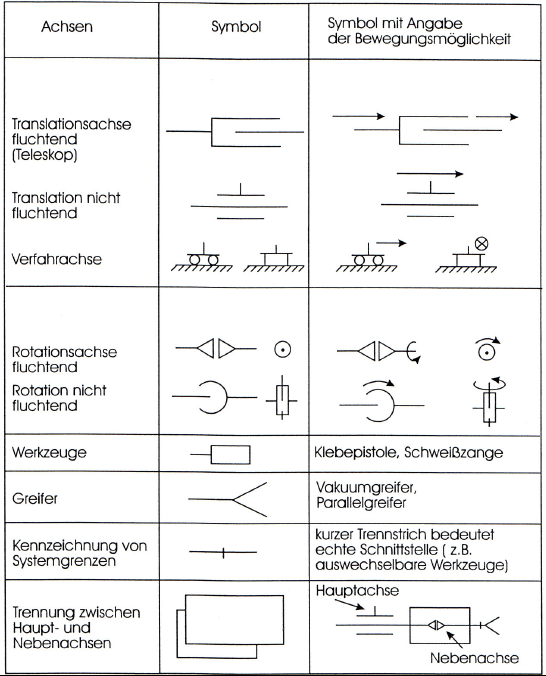
\includegraphics[width=10cm]{./bilder/symbole.png}
		\end{minipage}
		\begin{minipage}{8cm}
		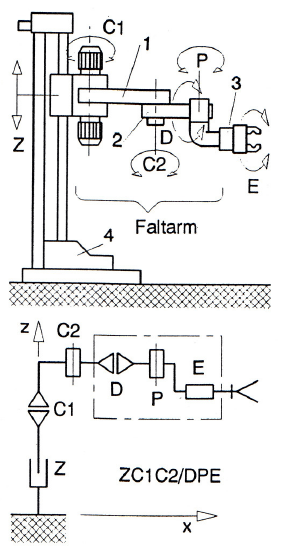
\includegraphics[width=5cm]{./bilder/symbole-bsp.png}
		\end{minipage}

	\subsection{Bewegungsarten}
		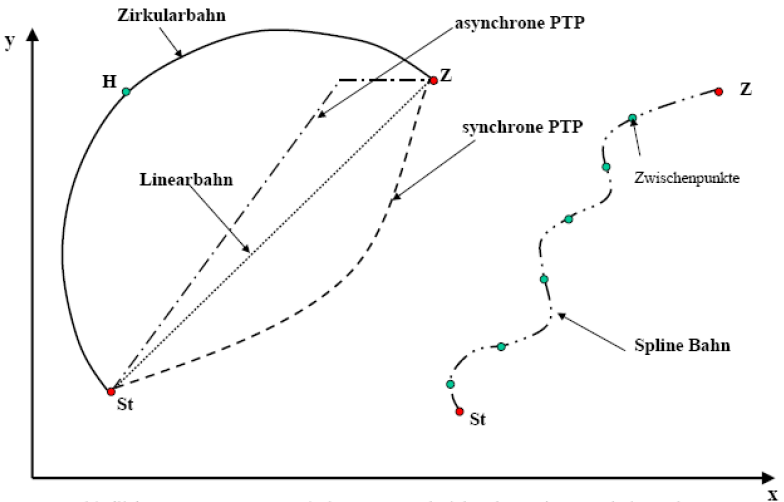
\includegraphics[width=10cm]{./bilder/bewegungsarten.png}
	
	\subsection{PTP-Synchron}
	\begin{minipage}{6cm}
		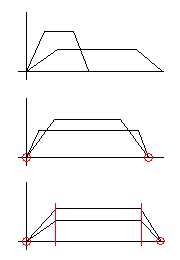
\includegraphics[width=5cm]{./bilder/synchron.png}
    \end{minipage}
	\begin{minipage}{12.5cm}
    	Asynchron PTP\\ \\ \\ \\ \\ \\
    	Synchron PTP\\ \\ \\ \\ \\ \\
    	Vollsynchron PTP\\
    \end{minipage}

	\subsection{Übersicht von Skript und Übungen}
	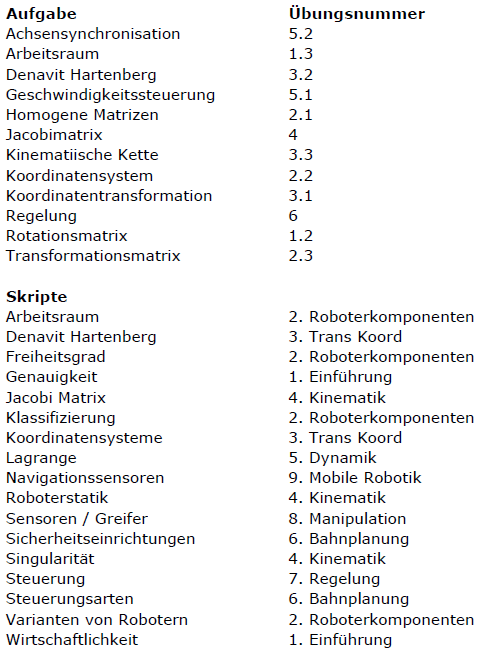
\includegraphics[width=10cm]{./bilder/uebersicht.png}